% !TeX spellcheck = en_US

\documentclass[justified,a4paper,
	nofonts,
	nobib
]{tufte-handout}

\title{Agricultural Plastic Covers---Source of Plastic Debris in Soil?}

\author{Zacharias Steinmetz}

\date{} % without \date command, current date is supplied

%\geometry{showframe} % display margins for debugging page layout

% A4 widths
% \marginparwidth = 1.94525in
% \textwidth = 4.21342in
% \pagewidth = 6.29707in

\usepackage{microtype}
\usepackage{graphicx} % allow embedded images
  \setkeys{Gin}{width=\linewidth,totalheight=\textheight,keepaspectratio}
  \graphicspath{proposal/} % set of paths to search for images

\usepackage{amsmath}  % extended mathematics
\usepackage{amsthm}
\usepackage{booktabs} % book-quality tables
\usepackage{tabulary}
\usepackage{multicol} % multiple column layout facilities
\usepackage{units}    % non-stacked fractions and better unit spacing
\usepackage[shortcuts]{extdash}
\usepackage[inline]{enumitem}
\usepackage{pgfgantt}
\usepackage{siunitx}
\usepackage{acro}
\usepackage{chemmacros}
\usepackage{chemfig}

\usepackage[
	backend=bibtex,
	natbib=true,
	style=ext-authoryear,
	date=year,
	maxnames=2,
	maxbibnames=10,
	dashed=false,
	clearlang=false,
	articlein=false,
	hyperref=true,
	giveninits=true,
	uniquename=init
]{biblatex}

% Add bibliography
\addbibresource{references.bib}

\usetikzlibrary{backgrounds}

\usepackage{fancyvrb} % extended verbatim environments
\fvset{fontsize=\normalsize}% default font size for fancy-verbatim environments

% Standardize command font styles and environments
\newcommand{\doccmd}[1]{\texttt{\textbackslash#1}}% command name -- adds backslash automatically
\newcommand{\docopt}[1]{\ensuremath{\langle}\textrm{\textit{#1}}\ensuremath{\rangle}}% optional command argument
\newcommand{\docarg}[1]{\textrm{\textit{#1}}}% (required) command argument
\newcommand{\docenv}[1]{\textsf{#1}}% environment name
\newcommand{\docpkg}[1]{\texttt{#1}}% package name
\newcommand{\doccls}[1]{\texttt{#1}}% document class name
\newcommand{\docclsopt}[1]{\texttt{#1}}% document class option name
\newenvironment{docspec}{\begin{quote}\noindent}{\end{quote}}% command specification environment

% Custom options

% Hyperref
\hypersetup{
	colorlinks=true,
	breaklinks=true,
	linktocpage=true,
	citecolor=InfDk,
	linkcolor=InfDk,
	urlcolor=InfRd,
	filecolor=InfRd
}

% BibLaTeX
% Lastname before firstname for all bib items
\DeclareNameAlias{sortname}{family-given}
\DeclareNameAlias{default}{family-given}
% Remove language fields and issn for articles
\AtEveryBibitem{%
	\clearlist{language}%
}
%\AtEveryBibitem{
%	\ifentrytype{article}{\clearfield{issn}}{}
%}
\renewcommand*{\bibfont}{\small}

% Ignore own contributions in reference list
\DeclareBibliographyCategory{ignore}

\addtocategory{ignore}{SteinmetzPlastic2016}
\addtocategory{ignore}{DavidQuantitative2018}
\addtocategory{ignore}{SteinmetzSimple2020}
\addtocategory{ignore}{ThomasSample2020}
\addtocategory{ignore}{SteinmetzAre2022}

\addtocategory{ignore}{CowgerOpenSpecy2021}
\addtocategory{ignore}{SteinmetzData2020}
\addtocategory{ignore}{SteinmetzEnvalysis2021}
\addtocategory{ignore}{SteinmetzData2022}

% Make \fullcite look like the bibliography
\DeclareCiteCommand{\fullcite}
{\usebibmacro{prenote}}
{\usedriver
	{\defcounter{maxnames}{10}}
	{\thefield{entrytype}}}
{\multicitedelim}
{\usebibmacro{postnote}}

%% Make own name bold
%\usepackage{xpatch}
%\makeatletter
%\newbibmacro*{name:bold}[2]{%
%	\edef\blx@tmp@name{\expandonce#1, \expandonce#2}%
%	\def\do##1{\ifdefstring{\blx@tmp@name}{##1}{\bfseries\listbreak}{}}%
%	\dolistloop{\boldnames}}
%\newcommand*{\boldnames}{}
%\makeatother
%
%\xpretobibmacro{name:family}{\begingroup\usebibmacro{name:bold}{#1}{#2}}{}{}
%\xpretobibmacro{name:given-family}{\begingroup\usebibmacro{name:bold}{#1}{#2}}{}{}
%\xpretobibmacro{name:family-given}{\begingroup\usebibmacro{name:bold}{#1}{#2}}{}{}
%\xpretobibmacro{name:delim}{\begingroup\normalfont}{}{}
%
%\xapptobibmacro{name:family}{\endgroup}{}{}
%\xapptobibmacro{name:given-family}{\endgroup}{}{}
%\xapptobibmacro{name:family-given}{\endgroup}{}{}
%\xapptobibmacro{name:delim}{\endgroup}{}{}
%
%\forcsvlist{\listadd\boldnames}
%{{Steinmetz, Z.}, {Steinmetz, Zacharias}, {Steinmetz, Z\bibinitperiod}}

% Enumerate options
\setlist[enumerate]{label={(\arabic*)}}

% Chemfig options
\setchemfig{
	atom sep=2.5em,
	cram width=2.5pt, cram dash width=0.75pt, cram dash sep=2.0pt
}
\renewcommand*\printatom[1]{\ensuremath{\mathsf{#1}}}

% DOI and CAS links
\newcommand*{\doi}[1]{\textsc{doi:} \texttt{\href{https://doi.org/#1}{#1}}}
\newcommand*{\cas}[2][CAS ]{#1\href{https://webbook.nist.gov/cgi/cbook.cgi?ID=#2}{#2}}

% Units options
\sisetup{
	detect-all,
	separate-uncertainty,
	tight-spacing = true,
	multi-part-units = single,
	list-units = single,
	range-units = single,
	range-phrase = --,
	exponent-product = \cdot,
	list-final-separator = {, and },
	table-alignment=left}
\DeclareSIUnit[number-unit-product = ]\percent{\char`\%}
\DeclareSIUnit\Molar{\text{\textsc{m}}}
\DeclareSIUnit\mz{\text{\textit{m/z}}}

% Acro options
\acsetup{
	single = 2,
	list/exclude = species
}

\NewAcroTemplate[list]{thesis}
{
	\acroheading
	\acropreamble
	\begin{description}[font=\normalfont,leftmargin=8em,style=nextline]
	\acronymsmapF
	{
		\item [ \acrowrite {short} \acroifT {alt} { / } \acrowrite {alt} ]
		\acrowrite {list}
		\acroifanyT {foreign,extra} {~(}
		\acrowrite {foreign}
		\acroifallT {foreign,extra} {,~}
		\acrowrite {extra}
		\acroifanyT {foreign,extra} {)}
		\acropagefill
		\acropages
		{ \acrotranslate {page} \nobreakspace }
		{ \acrotranslate {pages} \nobreakspace }
	}
	{ \item \AcroRerun }
	\end{description}
}

% Side- and marginnotes
\renewcommand{\thefootnote}{[\arabic{footnote}]}

\makeatletter
% Primitive input in tabular
\AddToHook{env/tabular/begin}{\let\input\@@input}
\makeatother

\hyphenation{
	mulch-ing
	bio-de-grad-able
	bio-deg-ra-da-tion
	deg-ra-da-tion
	solar-iza-tion
	metha-nol
	micro-plas-tic
	micro-plas-tics
	gra-vi-met-ry
	gra-vi-met-ric
	spec-tro-met-ry
	spec-tros-co-py
	pyro-ly-sis
	tri-chlo-ro-ben-zene
	hy-droxy-to-lu-ene
	poly-eth-yl-ene
	poly-pro-pyl-ene
	poly-sty-rene
	tere-phtha-late
	meth-acry-late
	poly-vi-nyl
	poly-but-yl-ene
	poly-hy-droxy-butyrate
	poly-tetra-fluoro-eth-yl-ene
	poly-am-ide
	chro-ma-tog-ra-phy
	eth-yl-ene
	di-oxy-thio-phene
	me-thyl
	am-mo-nium
	mod-el
	Er-ke-ko-glu
	Chan-nell-Butch-er
	Bon-fer-ro-ni
	Schacht-schabel
	Marsch-ner
	ethyl-hexyl-phtalate
}
% !TeX spellcheck = en_US

% Soil chemistry
\DeclareAcronym{som}{
	short = SOM,
	long = soil organic matter
}
\DeclareAcronym{Corg}{
	short = C\textsubscript{org},
	long = organic carbon
}
\DeclareAcronym{ec}{
	short = EC,
	long = electrical conductivity
}
\DeclareAcronym{uv}{
	short = UV,
	long = ultraviolet,
	long-plural = ,
	long-indefinite = an
}
\DeclareAcronym{ir}{
	short = IR,
	long = infrared,
	long-plural = ,
	long-indefinite = an,
	short-indefinite = an
}
\DeclareAcronym{par}{
	short = PAR,
	long = photosynthetically active radiation
}
\DeclareAcronym{kow}{
	short = $K_{ow}$,
	long = octanol--water partitioning coefficient
}

% Chemicals
\DeclareAcronym{pe}{
	short = PE,
	long = polyethylene
}
\DeclareAcronym{ldpe}{
	short = LDPE,
	long = low\-/density polyethylene,
	short-indefinite = an
}
\DeclareAcronym{lldpe}{
	short = LLDPE,
	long = linear low\-/density polyethylene,
	short-indefinite = an
}
\DeclareAcronym{hdpe}{
	short = HDPE,
	long = high\-/density polyethylene
}
\DeclareAcronym{pa}{
	short = PA,
	long = polyamide
}
\DeclareAcronym{pc}{
	short = PC,
	long = polycarbonate
}
\DeclareAcronym{pp}{
	short = PP,
	long = polypropylene
}
\DeclareAcronym{ps}{
	short = PS,
	long = polystyrene
}
\DeclareAcronym{pet}{
	short = PET,
	long = polyethylene terephthalate
}
\DeclareAcronym{pmma}{
	short = PMMA,
	long = poly(methyl methacrylate)
}
\DeclareAcronym{twp}{
	short = TWP,
	long = tire wear particles
}
\DeclareAcronym{pu}{
	short = PU,
	long = polyurethane
}
\DeclareAcronym{abs}{
	short = ABS,
	long = acrylonitrile butadiene styrene,
	short-indefinite = an,
	long-indefinite = an
}
\DeclareAcronym{pvc}{
	short = PVC,
	long = polyvinyl chloride
}
\DeclareAcronym{pbt}{
	short = PBT,
	long = polybutylene terephthalate
}
\DeclareAcronym{pbs}{
	short = PBS,
	long = polybutylene sebacate
}
\DeclareAcronym{pbat}{
	short = PBAT,
	long = polybutylene adipate terephthalate
}
\DeclareAcronym{pla}{
	short = PLA,
	long = polylactic acid
}
\DeclareAcronym{eva}{
	short = EVA,
	long = ethylene vinyl acetate,
	short-indefinite = an,
	long-indefinite = an
}
\DeclareAcronym{eba}{
	short = EBA,
	long = ethylene butyl acrylate,
	short-indefinite = an,
	long-indefinite = an
}
\DeclareAcronym{ptfe}{
	short = PTFE,
	long = polytetrafluoroethylene
}
\DeclareAcronym{pae}{
	short = PAE,
	long = phthalic acid ester
}
\DeclareAcronym{dep}{
	short = DEP,
	long = diethyl phthalate
}
\DeclareAcronym{dbp}{
	short = DBP,
	long = dibutyl phthalate
}
\DeclareAcronym{dehp}{
	short = DEHP,
	long = bis(2-ethylhexyl) phthalate
}
\DeclareAcronym{tcb}{
	short = TCB,
	long = {1,2,4}-trichlorobenzene
}
\DeclareAcronym{dcm}{
	short = DCM,
	long = dichloromethane
}
\DeclareAcronym{hfip}{
	short = HFIP,
	long = hexafluoroisopropanol
}
\DeclareAcronym{thf}{
	short = THF,
	long = tetrahydrofuran
}
\DeclareAcronym{tfa}{
	short = TFA,
	long = trifluoroacetic acid
}
\DeclareAcronym{bht}{
	short = BHT,
	long = butylated hydroxytoluene
}
\DeclareAcronym{pedot}{
	short = PEDOT,
	long = poly({3,4}\-/ethylenedioxythiophene)
}
\DeclareAcronym{tmsh}{
	short = TMSH,
	long = trimethylsulfonium hydroxide
}
\DeclareAcronym{tmah}{
	short = TMAH,
	long = tetramethylammonium hydroxide
}
\DeclareAcronym{bstfa}{
	short = BSTFA,
	long = {\textit{N},\textit{O}\--bis(trimethylsilyl)trifluoroacetamide}
}
\DeclareAcronym{spt}{
	short = SPT,
	long = sodium polytungstate
}


% Instrumental analytics
\DeclareAcronym{mwe}{
	short = MWE,
	long = microwave\-/induced extraction
}
\DeclareAcronym{use}{
	short = USE,
	long = ultrasonic extraction,
	long-indefinite = an
}
\DeclareAcronym{ase}{
	short = ASE,
	long = accelerated solvent extraction,
	short-indefinite = an,
	long-indefinite = an
}
\DeclareAcronym{spe}{
	short = SPE,
	long = solid phase extraction,
	short-indefinite = an
}
\DeclareAcronym{sec}{
	short = SEC,
	long =  size exclusion chromatography
}
\DeclareAcronym{gpc}{
	short = GPC,
	long =  gel permeation chromatography
}
\DeclareAcronym{gc}{
	short = GC,
	long = gas chromatograph
}
\DeclareAcronym{ms}{
	short = MS,
	long = mass spectrometer,
	short-indefinite = an
}
\DeclareAcronym{tof}{
	short = TOF,
	long = time-of-flight
}
\DeclareAcronym{ei}{
	short = EI,
	long = electron ionization,
	short-indefinite = an,
	long-indefinite = an
}
\DeclareAcronym{ssl}{
	short = S/SL,
	long = split\slash splitless,
	short-indefinite = an
}
\DeclareAcronym{gc-ms}{
	short = GC/MS,
	long = gas chromatography\slash mass spectrometry
}
\DeclareAcronym{ega}{
	short = EGA,
	long = evolved gas analysis
}
\DeclareAcronym{py-gc-ms}{
	short = Py-GC/MS,
	long = pyrolysis\-/gas chromatography\slash mass spectrometry
}
\DeclareAcronym{ted-gc-ms}{
	short = TED-GC/MS,
	long = thermal extraction and desorption\-/gas chromatography\slash mass spectrometry
}
\DeclareAcronym{tga-ms}{
	short = TGA/MS,
	long = thermogravimetry\slash mass spectrometry
}
\DeclareAcronym{sem}{
	short = SEM,
	long = secondary electron multiplier,
	short-indefinite = an
}
\DeclareAcronym{dsc}{
	short = DSC,
	long = differential scanning calorimetry
}
\DeclareAcronym{lc}{
	short = LC,
	long = liquid chromatography
}
\DeclareAcronym{lc-ms}{
	short = LC/MS,
	long = liquid chromatography\slash mass spectrometry
}
\DeclareAcronym{ftir}{
	short = FTIR,
	long = Fourier transformed infrared
}
\DeclareAcronym{atr}{
	short = ATR,
	long = attenuated total reflection
}
\DeclareAcronym{fpa}{
	short = FPA,
	long = focal plane array,
	short-indefinite = an
}
\DeclareAcronym{esem}{
	short = ESEM,
	long = environmental scanning electron microscopy,
	short-indefinite = an,
	long-indefinite = an
}
\DeclareAcronym{hnmr}{
	short = \textsuperscript{1}H NMR,
	long = \textsuperscript{1}H nuclear magnetic resonance spectroscopy
}
\DeclareAcronym{tof-sims}{
	short = TOF/SIMS,
	long = time-of-flight\slash secondary ion mass spectrometry
}
\DeclareAcronym{tga}{
	short = TGA,
	long = thermogravimetric analysis,
	long-plural-form = thermogravimetric analyses
}
\DeclareAcronym{dtg}{
	short = DTG,
	long = derivative thermogravimetry,
	long-plural-form = derivative thermogravimetries
}
\DeclareAcronym{nir}{
	short = NIR,
	long = near infrared
}
\DeclareAcronym{rt}{
	short = RT,
	long = retention time,
	short-indefinite = an
}
\DeclareAcronym{ri}{
	short = RI,
	long = retention index,
	long-plural-form = retention indices,	
	short-indefinite = an
}
\DeclareAcronym{sim}{
	short = SIM,
	long = selected ion monitoring
}
\DeclareAcronym{lod}{
	short = LOD,
	long = limit of detection,
	long-plural-form = limits of detection,
	short-indefinite = an
}
\DeclareAcronym{loq}{
	short = LOQ,
	long = limit of quantification,
	long-plural-form = limits of quantification,
	short-indefinite = an
}
\DeclareAcronym{snr}{
	short = SNR,
	long = signal\-/to\-/noise ratio,
	short-indefinite = an
}
\DeclareAcronym{sse}{
	short = SSE,
	long = signal suppression\slash enhancement,
	short-indefinite = an
}
\DeclareAcronym{tic}{
	short = TIC,
	long = total ion current
}
\DeclareAcronym{tml}{
	short = TML,
	long = thermal mass loss,
	long-plural-form = thermal mass losses
}

%Stats
\DeclareAcronym{sd}{
	short = SD,
	long = standard deviation,
	short-indefinite = an
}
\DeclareAcronym{rsd}{
	short = RSD,
	long = relative standard deviation,
	short-indefinite = an
}
\DeclareAcronym{rse}{
	short = RSE,
	long = relative standard error,
	short-indefinite = an
}
\DeclareAcronym{ci}{
	short = CI,
	long = confidence interval
}
\DeclareAcronym{pca}{
	short = PCA,
	long = principal component analysis
}
\DeclareAcronym{anova}{
	short = ANOVA,
	long = analysis of variance,
	long-plural-form = analyses of variance,
	short-indefinite = an,
	long-indefinite = an
}
\DeclareAcronym{aic}{
	short = AIC,
	long = akaike information criterion,
	long-plural-form = akaike information criteria,
	short-indefinite = an,
	long-indefinite = an
}


\begin{document}

\maketitle% this prints the handout title, author, and date

\begin{abstract}
\noindent\textit{Abstract}~~
Agricultural fields are covered with plastic films to make crop growth more economical. While in use, however, plastic covers may emit plastic debris into the field’s surrounding. This pathway of plastic fate is still largely understudied due to the lack of analytical methods for the quantification of microplastics in soil.
Within the scope of my dissertation, I aim to scrutinize the agricultural use of plastic covers and analytical methods for plastic analyses in order to develop a robust method for plastic quantification in agricultural soil. The new method will be applied in a field screening study to assess the extent of plastic pollution in and around fields covered with plastic films. Thereby, I intend to contribute to a better understanding of the occurrence and fate of plastic debris in terrestrial ecosystems.
\end{abstract}

\section{Scientific Background}\label{sec:background}

Covering soil with plastic films has become a widely applied agricultural practice for its economic benefits such as improving crop yields and crop quality, managing harvest times, and increasing water use efficiency \citep{LamontPlastic1993}. The most common materials used are \ac{pe} foils and \ac{pp} fleeces in various thicknesses.
Although made to last for \numrange{3}{5} years, wind, heavy machinery, animals, or \ac{uv} irradiation are likely to disintegrate parts of the plastic covers into particles smaller than \SI{5}{\milli\meter} \citep{Scarascia-MugnozzaPlastic2011}, called microplastics \citep{HartmannAre2019}. This supposition raised a discussion about agricultural plastic covers acting as a potential source of plastic debris in the environment \citep{HurleyFate2018}.
However, the actual contribution of agricultural plastic covers to plastic pollution is virtually unknown and has not yet been discriminated from other potential sources like aerial deposition, littering, or tire debris \citep{HurleyFate2018}.

Developing a better understanding of the occurrence and fate of plastic debris in the terrestrial environment requires analytical methods for reliable microplastic quantification \citep{BlasingPlastics2018,HeMicroplastics2018}.
So far, the majority of studies have assessed microplastics in water or sediment, and mostly relied on optical detection by \ac{ftir} or Raman microspectroscopy \citep{RennerAnalytical2018}. Both techniques require extensive sample preparation to separate plastic particles from sample matrix without losing analyte \citep{HurleyValidation2018}. With more complex matrices such as soil or organic tissues, microplastic separation becomes increasingly tedious and prone to false detections from interfering matrix. While this complicates the quantification of plastic particles, optical techniques provide additional information on particle shapes and sizes. \citet{ScheurerMicroplastics2018} were the first who successfully developed and applied a method for the quantification of microplastics in soil using a combination of density separation and oxidative matrix digestion followed by \ac{ftir} spectroscopy. With their procedure, the authors obtained recoveries of \SIrange{93}{98}{\percent} and found plastic concentrations in Swiss floodplain soils averaging \SI{5}{\milli\gram\per\kilogram}. However, they did not state any \acp{lod} or \acp{loq}.

An alternative approach is thermoanalytical techniques such as \ac{ted-gc-ms} \citep{DumichenFast2017} or \ac{py-gc-ms} \citep{FischerSimultaneous2017}. The methods are based on thermal decomposition of polymers and their quantification via characteristic pyrolysis products. In contrast to optical methods, thermoanalytical techniques are assumed to be more robust against impurities from sample matrix. However, interferences may occur when pyrolysis products in plastic and matrix are identical. In addition, thermoanalytical measurements are typically restricted to sample amounts of \SIrange{0.1}{100}{\milli\gram} which puts high requirements on sample homogeneity. This challenge might be overcome by combining simple sample preparation techniques as usually applied prior to optical detection with \ac{py-gc-ms}.

\section{Research Objective}\label{sec:objective}

With this dissertation project, I aim to contribute to a better process understanding of the fate of plastic debris in agricultural ecosystems by assessing to what extent agricultural plastic covers act as a source of plastic debris in soil.

This
\begin{enumerate*}
	\item requires the development of a reliable method for a time- and cost\-/effective sample preparation and thermoanalytical quantification of microplastics in soil. Due to the widespread use of \ac{pe} and \ac{pp}, method development focuses on these two polymers.
	Subsequently, \item soils sampled within and around agricultural fields covered with plastic films will be analyzed for \ac{pe} and \ac{pp} to elucidate the distribution of microplastics at field level. Whereas a directed concentration gradient of microplastics from the field center to its periphery would support the assumption of plastic covers contributing to increased microplastic concentrations in soil, an undirected gradient would suggest another source of pollution such as littering. A uniform distribution, however, may be an indicator for aerial deposition. In addition, field borders are expected to be particular hotspots for microplastics due to mechanical stress subjected to plastic covers by weighting them down with soil or sandbags.
\end{enumerate*}

\section{Working Program}\label{sec:methods}

\subsection{Current trends in plasticulture and plastic analytics}

In order to acquire an in-depth understanding of current agricultural practices involving plastic mulching and state-of-the-art analytical methods, two literature reviews were conducted.

The literature review on plastic mulching\sidenote[][-3\baselineskip]{Published as \fullcite{SteinmetzPlastic2016}.} critically discussed the current understanding of the environmental impact of plastic
mulch use by linking knowledge of agricultural benefits and research on the life cycle of plastic mulches with direct and indirect implications for long-term soil quality and ecosystem services. By reviewing current analytical methods\sidenote{Published as \fullcite{ThomasSample2020}.} we disentangled the variety of state-of-the-art
sample preparation techniques for heterogeneous solid matrices to identify and discuss
best-practice methods for soil-focused microplastic analyses.

\subsection{Developing Analytical Methods for the Quantification of Plastic Debris in Soil}\label{sec:methods-development}

%\begin{figure}[t]
%	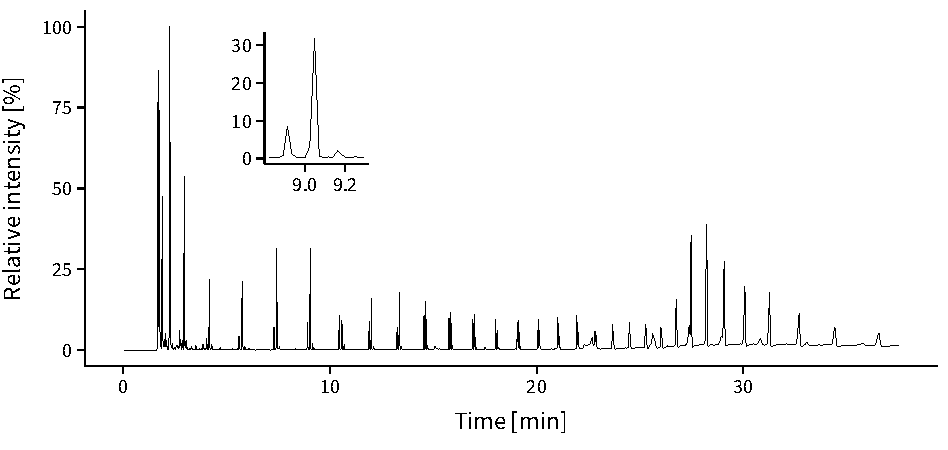
\includegraphics{proposal/pyrogram}
%	\caption{Pyrolysis of \acl{pe} in a reference loamy sand (LUFA type 2.2, Speyer, Germany) at \SI{700}{\degreeCelsius} \citetext{preliminary data}.}
%	\label{fig:pyrogram}%
%\end{figure}

While total polymer contents can be easily assessed via \ac{tga-ms}\sidenote[][-2.5\baselineskip]{Published as \fullcite{DavidQuantitative2018}.}, \ac{py-gc-ms} is required for polymer\-/specific quantification \citep{BeckerQuantification2020}. To this end, method development first focused on the preparation of an operating procedure for routine \ac{py-gc-ms} measurements using a Pyroprobe 6150 (CDS Analytical, Oxford, US) coupled with a GC Trace Ultra with a DSQII-MSD (Thermo Fisher Scientific, Bremen, Germany). This included the identification of characteristic \ac{pe} and \ac{pp} pyrolysis products that did not interfere with the soil matrix and yield sufficiently stable peak intensities for subsequent quantification.

Calibration curves were prepared by dissolving \ac{pe} and \ac{pp} in 1,2,4\-/trichlorobenzene with \SI{0.015}{\percent} butylated hydroxytoluene. The solvent is usually used for \ac{sec} of polymers \citep{BivensPolymertoSolvent2016}. Dissolution of plastic particles significantly facilitated the preparation of defined plastic concentrations for calibration curves. Calibration curves were assessed for linearity and sensitivity of peak responses before lowering concentrations for the optimization of \acp{lod} and \acp{loq}\sidenote{Published as \fullcite{SteinmetzSimple2020}.}.

Subsequently, agricultural reference soils were spiked with \ac{pe} and \ac{pp} to be tested for their susceptibility to the (bio)\-chemical pretreatments summarized in Table~\ref{tab:extraction}. As for the preparation of calibration curves, dissolution of plastic particles with 1,2,4-trichlorobenzene \citep{BivensPolymertoSolvent2016} and extraction from may be particularly promising to account for the heterogeneous distribution of plastic particles in soil while reducing the total sample amount subjected to pyrolysis. In addition, samples may be spiked with deuterated \ac{ps} as internal standard to increase the repeatability of the method.

\begin{table}
	\centering\footnotesize
	\caption{Potential (bio)chemical pretreatments.}\label{tab:extraction}
	\begin{tabulary}{\linewidth}{LLL}
		\toprule
		Method & Chemicals & Reference \\
		\midrule
		Dissolution of plastic particles & 1,2,4-Trichlorobenzene + \SI{0.015}{\percent} butylated hydroxytoluene & \citealp{BivensPolymertoSolvent2016} \\
		Matrix oxidation & \ch{H2O2} & \citealp{NuelleNew2014} \\
		& Fenton reagent & \\
		Density fractionation & \ch{ZnCl2} & \citealp{ImhofPigments2016} \\
		Acid digestion & \ch{HNO3} & \citealp{ScheurerMicroplastics2018} \\
		Enzymatic digestion & Protease, chitinase & \citealp{LoderEnzymatic2017} \\
		Sequential purification & Sodium dodecyl sulfate with enzymatic digestion and \ch{H2O2} & \citealp{FischerSimultaneous2017} \\
		\bottomrule
	\end{tabulary}
\end{table}

\subsection{Screening Study: Are Agricultural Plastic Films a Source for Plastic Particles in Soil?}

\begin{marginfigure}
	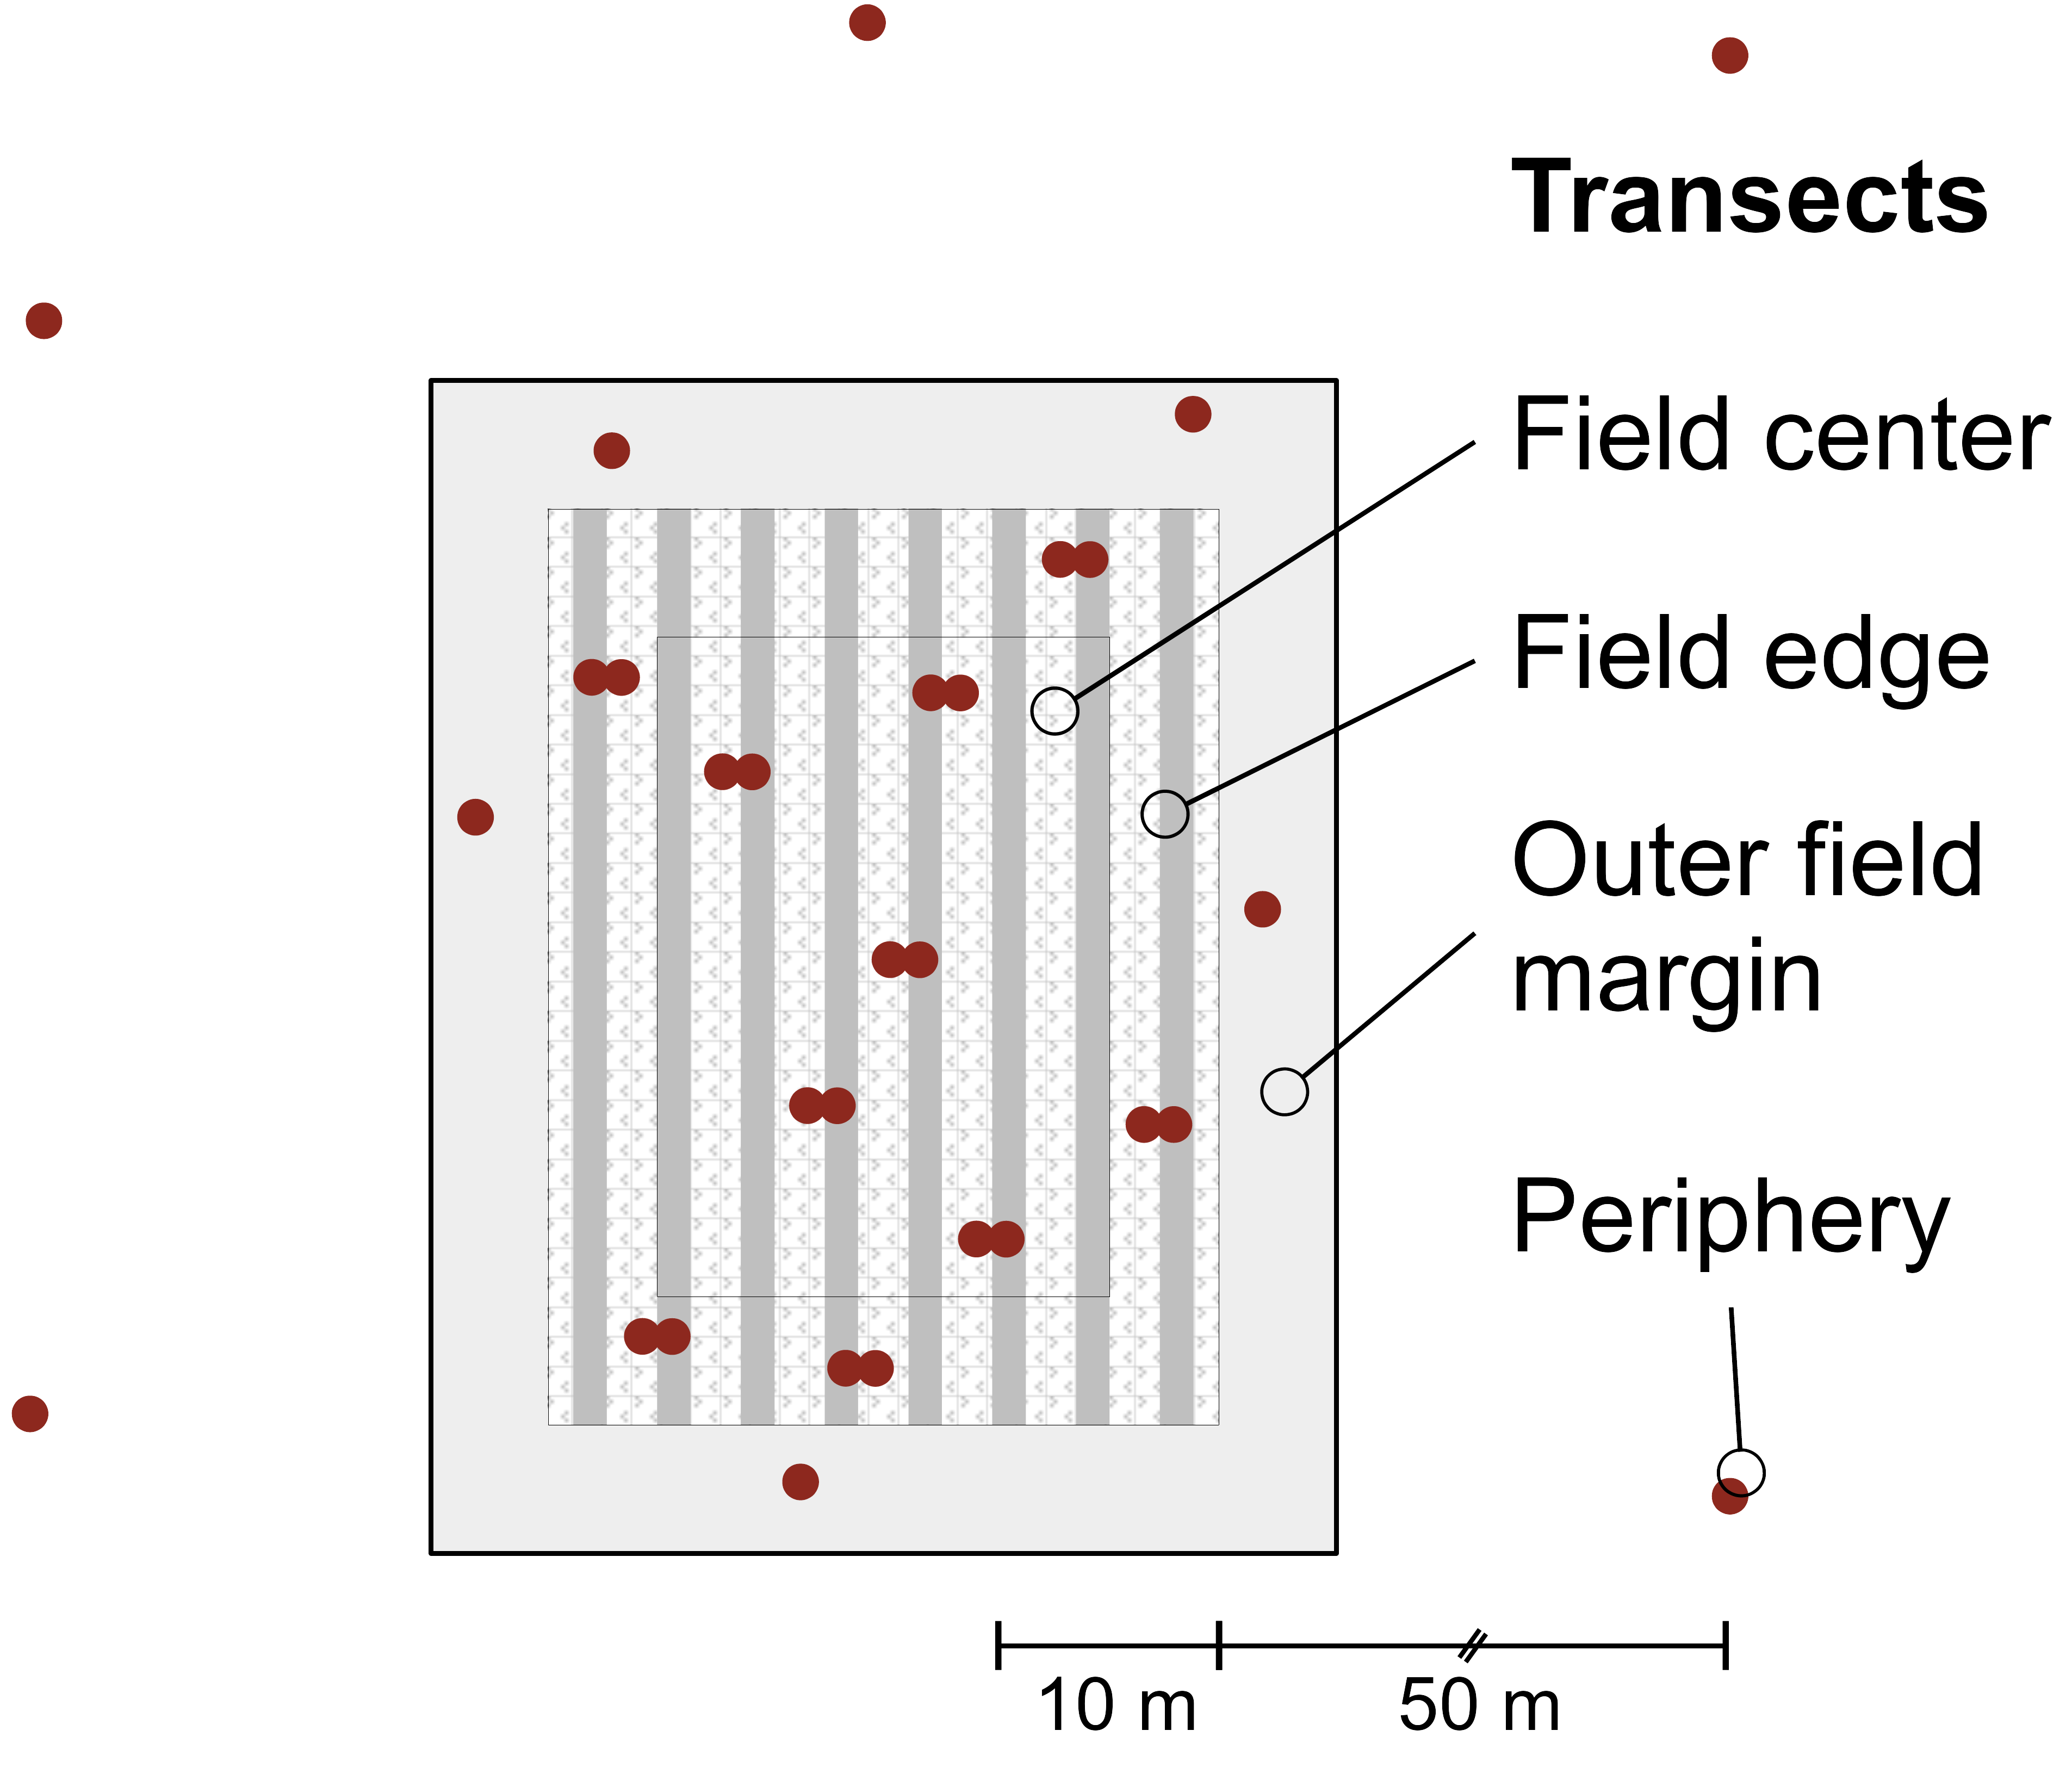
\includegraphics{proposal/field}
	\caption{Randomized sampling scheme for one exemplary plot with $n$ = 5 samples (\SIrange{0}{5}{\centi\meter} depth) per transect; within the cultivated field, ridges and furrows are sampled separately.}
	\label{fig:field}%
\end{marginfigure}

\begin{table}[b]
	\centering\footnotesize
	\caption{Sampling sites.}\label{tab:sites}
	\begin{tabular}{lllll}
		\toprule
		Site & Cover & Polymer & Cultivation & Location \\
		\midrule
		1 & Fleece under perforated foil & \acs{pp}, \acs{pe} & Strawberry & Offenbach \\
		3 & Black mulch under fleece & \acs{pe}, \acs{pp} & Strawberry & Offenbach \\
		4 & Black mulch & \acs{pe} & Strawberry & Offenbach \\
		9 & Fleece under perforated foil & \acs{pp}, \acs{pe} & Lettuce & Schifferstadt \\
		12 & Perforated foil & \acs{pe} & Rhubarb & Landau  \\
		13 & Fleece under perforated foil & \acs{pe}, \acs{pe} & Cabbage & Schifferstadt \\
		14 & Perforated foil & \acs{pe} & Rhubarb & Landau \\
		15 & Perforated foil & \acs{pe} & Rhubarb & Landau \\
		\bottomrule
	\end{tabular}
\end{table}

In order to screen agricultural fields covered with plastic films for their contribution to microplastic pollution and to better understand the distribution of microplastics at field level, $n = 8$ sampling sites in Palatinate, Germany (Table~\ref{tab:sites}), were be subdivided into \num{4} transects as shown in Figure~\ref{fig:field}. Sampling spots were randomly selected for each transect. In cultivated field transects, namely field centers and inner field edges, plant rows (ridges) and track rows (furrows) were sampled separately. Topsoil (\SIrange{0}{5}{\centi\meter} depth) were sampled shortly after retrieval of plastic covers in spring 2018. Samples will be analyzed for plastic particles as outlined in Section~\ref{sec:methods-development}.

\subsection{Schedule}

The dissertation project follows the schedule shown in Figure~\ref{fig:ganttchart}, including a research stay in Finland for additional training of analytical and extraction techniques.

\begin{figure*}
	\begin{ganttchart}[
	expand chart=\textwidth,
	y unit title=8mm,
	y unit chart=6mm,
	bar top shift=-0.1, bar height=0.6,
	vgrid={{draw=none}, {draw=none}, {dotted, gray}},
	canvas/.style={draw=none},
	link/.style={-latex},
	link/.append style={color=InfDk},
	time slot format=isodate-yearmonth,
	time slot unit=month,
	title label font=\normalsize\sffamily,
	group label font=\small\sffamily\bfseries\color{InfDk},
	group/.append style={fill=InfDk},
	bar label font=\footnotesize\sffamily,
	milestone label font=\small\sffamily\bfseries\color{InfDk},
	milestone/.append style={fill=InfDk, color=InfDk},
	]{2018-01}{2021-12}
	\gantttitlecalendar{year} \\
	\ganttgroup[name=g0]{Literature review}{2018-01}{2020-07} \\
	\ganttbar[inline]{Plastic covers}{2017-07}{2018-01} 
	\ganttbar[inline]{Analytical methods}{2018-06}{2019-02}
	\ganttbar[inline]{Soil sample preparation}{2019-07}{2020-06} \\
	\ganttmilestone[name=m0]{}{2020-09}
	\begin{scope}[on background layer]
		\ganttlink{g0}{m0}
	\end{scope}
	\\
	\ganttgroup[name=g1]{Analytical methods}{2018-01}{2019-11} \\
	\ganttbar[inline, bar inline label node/.append style={left=3mm}]{Method development}{2018-03}{2018-03}
	\ganttbar[inline]{\acs{tga-ms}}{2018-03}{2018-12}
	\ganttbar[inline]{\acs{py-gc-ms}}{2019-02}{2019-10} \\
	\ganttbar[inline]{Plastic extraction from soil}{2018-08}{2019-07} \\
	\ganttbar[inline, bar inline label node/.append style={left=5mm}]{Analytical training\textsuperscript{\textdagger}}{2019-06}{2019-08}
	\ganttbar[inline]{}{2019-06}{2019-08}
	\ganttmilestone[name=m1]{}{2020-01}
	\begin{scope}[on background layer]
		\ganttlink{g1}{m1}
	\end{scope}
	\\
	\ganttgroup[name=g2]{Screening study}{2018-04}{2021-01} \\
	\ganttbar[inline, bar inline label node/.append style={left=3mm}]{Soil sampling}{2018-04}{2018-04} \\
	\ganttbar[inline, bar inline label node/.append style={left=5mm}]{Soil characterization}{2018-05}{2018-07} \\
	\ganttbar[inline]{Plastic analyses}{2020-02}{2020-12}
	\ganttmilestone[name=m2]{}{2021-03}
	\begin{scope}[on background layer]
		\ganttlink{g2}{m2}
	\end{scope}
	\\
	\ganttgroup[name=gf]{Synthesis}{2021-03}{2021-07} \\
	\ganttmilestone[name=mf, inline, milestone inline label node/.append style={left=5mm}]{Thesis submission}{2021-09}
	\begin{scope}[on background layer]
		\ganttlink{gf}{mf}
	\end{scope}
\end{ganttchart}
	\caption{Research schedule of the dissertation project subdivided into three working packages; \textsuperscript{\textdagger} includes additional training on analytical and extraction techniques at Lappeenranta University of Technology, Finland.}
	\label{fig:ganttchart}%
\end{figure*}

\section{Outlook}\label{sec:outlook}

The availability of a reliable method for the quantification of \ac{pe} and \ac{pp} microplastics in soil would considerably contribute to the advancement of microplastic research. Knowing microplastic concentrations in soil and understanding the fate of microplastic particles in the environment will enable a realistic risk assessment of microplastics and communication of these risks to farmers and consumers.

\begin{fullwidth}
	\printbibliography[notcategory=ignore]
\end{fullwidth}

\end{document}
